\chapter{Development}

\label{ch:conclusions}

\section{Introduction}

As explained in the design chapter, this project includes three deliverables. So the development will include; a Mac app dashboard, Perfect web-server and CocoaPods framework. Using the "tree-shaped" methodology the web-server was split up into their separate sections which include development, testing, and run. Then each service was design, developed and testing before moving up the tree. The development then broken up into phases, this way the project can be kept on track on what has been completed and whats left to do.

\begin{enumerate}
  \item Services Development
  \item Integrate into Live App
  \item Dashboard Development
  \item CocoaPod Framework 
\end{enumerate}

\section{Services Development}

Each service had its own flask application along with Playground app. This made is easy to decide whether or not it was possible to implement each service into the project.

\subsubsection{Database storage}

The database storage required an object role model (ORM) which is a powerful method for designing and querying database models at the conceptual level, where the application is described in terms easily understood by non-technical database developers. It is a technique for converting data between incompatible type systems in object-oriented programming languages. The ORM was developed using Playground tool, where the creation of objects and parsing into JSON objects. The functionality of the ORM is to create a new object, parse it and send to the server, and be able to bring all objects back from the server. Extra functionality was added to be able to send filters.

\begin{figure}[!h]
    \caption{Storage Sequence Standard}
    \centering
    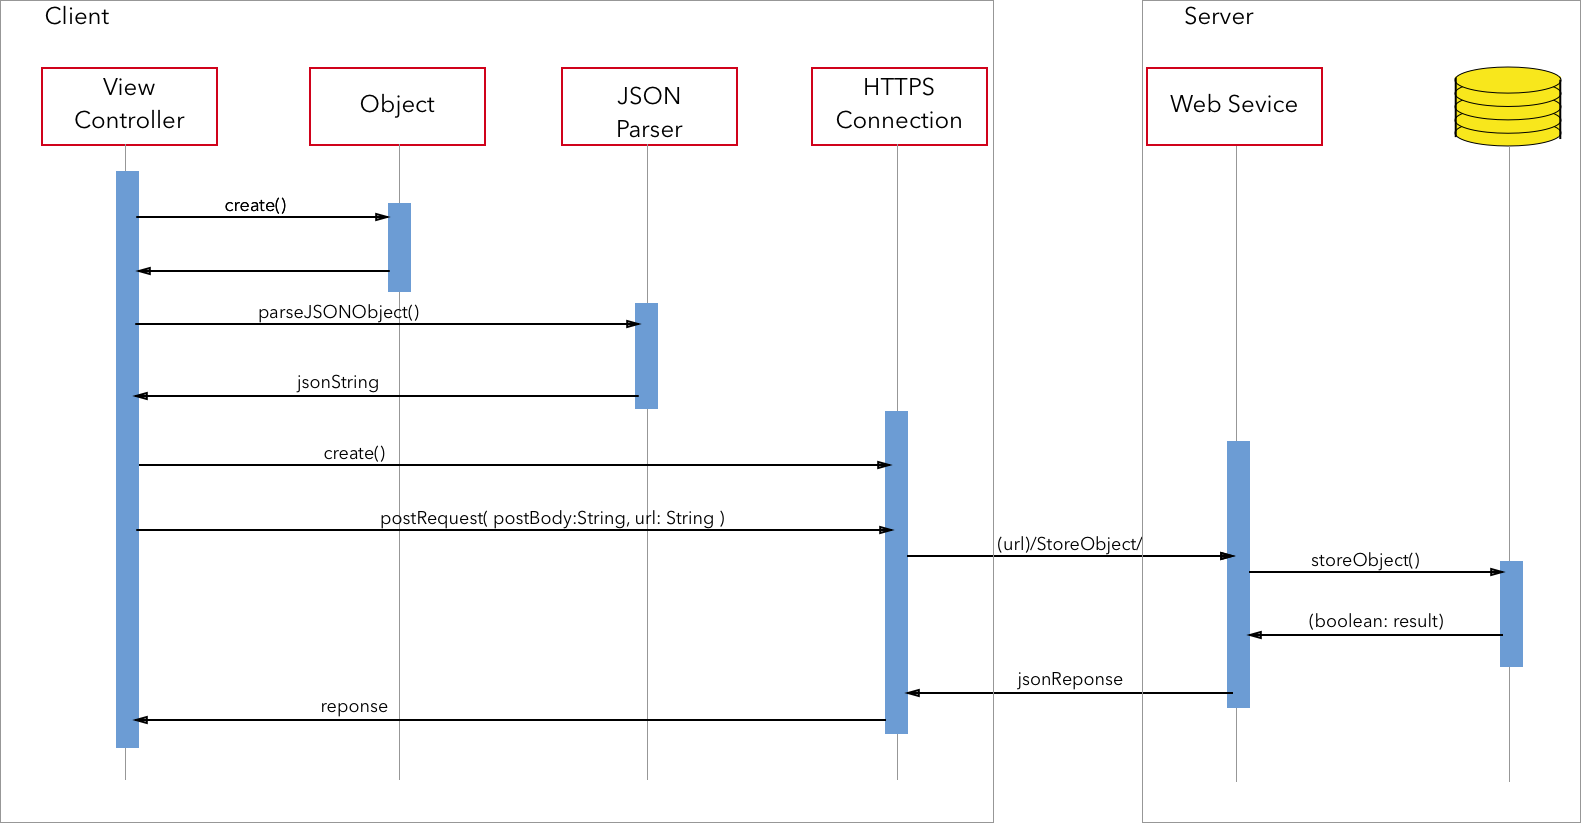
\includegraphics[width=100mm]{images/services/storage_sequence_current}
    \label{fig:storage_old}
\end{figure}


\begin{figure}[!h]
    \caption{Storage Sequence New}
    \centering
    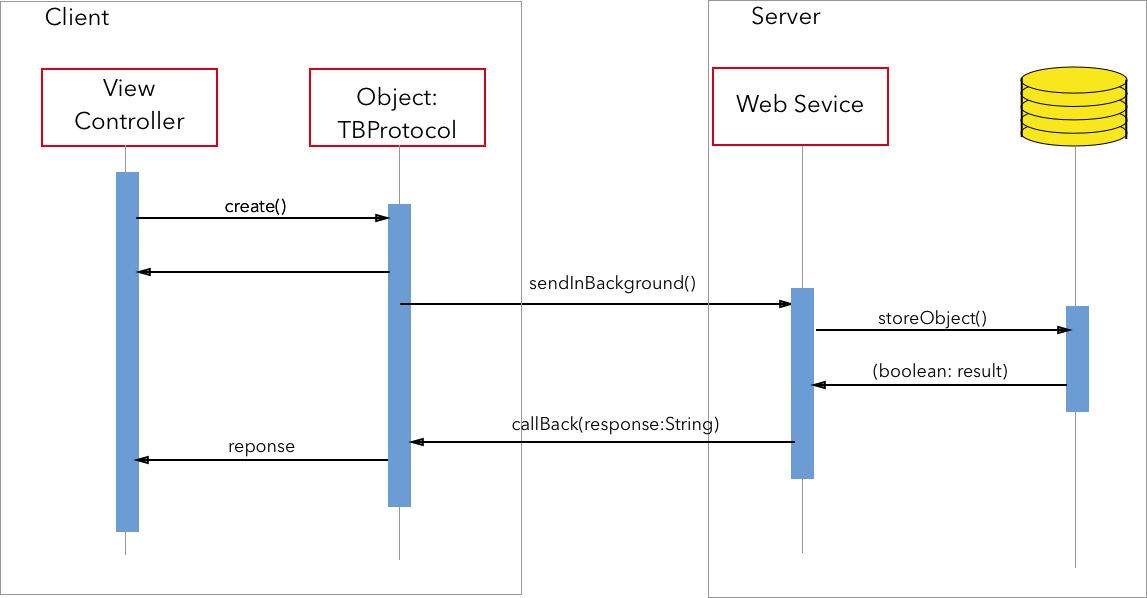
\includegraphics[width=100mm]{images/services/storage_sequence}
    \label{fig:storage_new}
\end{figure}

The two figures above show the difference to developing the standard way, with the developing having to create a JSON parser and then set-up a HTTPS connection to send it to the server in Fig \ref{fig:storage_old} . The new way in Fig \ref{fig:storage_new} using the project's storage protocol involves the developer only having to create the object, then using the objects functionality to send it to the server.

\subsubsection{Push notifications}


\subsubsection{Analytics}


\subsubsection{Backup}


\subsubsection{Self hosted}


\subsubsection{Remote Configuration}


\subsubsection{A/B Testing}


\subsubsection{Live Database}


\subsubsection{Exception catching}


\section{Integrate into Live App}

For some parts of project, an already developed and published app called DIT-Timetable was used to add in the services, to test if Apple would allow it through. The services include remote configuration and language choice. Due to Apple's strict guidelines, the remote configuration was developed into the DIT-Timetable app into two stages, then each stage had a build and published.

\subsubsection{Phase 1}
This phase included just the basic remote configuration, with the capability of updating text such as page title, and label values. Apple did approve this phase, and while the app live, using the iPad prototyping app the text values were able to be changed. 

\subsubsection{Phase 2}

Phase 2 gave the ability to adjust user interface values such as text colour, text size and user interaction enabling/disabling. This also been approved by Apple giving it a go ahead to be completely integrated into the project.  

\section{Dashboard Development}

The dashboard was originally going to be created as an iPad app, but after some thought that not all mobile developers can be expected to own an iPad, the dashboard was developed as a Mac App. 

\section{CocoaPod Framework}

The CocoaPod was left to last to development, as all the test cases used in the Playground could be brought over and adjusted to fit the framework. After the CocoaPod was finished, a test project was created for external professional mobile developers to use and give some feedback.